\documentclass[12pt,a4paper]{article}
\usepackage[T2A]{fontenc}
\usepackage[utf8]{inputenc}
\usepackage[russian]{babel}
\usepackage{amsmath}
\usepackage{amssymb}
\usepackage{graphicx}
\usepackage{floatrow}
\usepackage{booktabs}
%\usepackage{wrapfig}
\usepackage{lipsum}
%\usepackage{subcaption}
\usepackage{fancyhdr}


%multi-column
%\multicolumn{number cols}{align}{text} % align: l,c,r

%multi-row
\usepackage{multirow}

\newcommand{\figref}[1]{(См. рис. \ref{#1})}
\newcommand{\secref}[1]{(См. раздел. \ref{#1})}

\newcommand{\e}[1]{\text{$\cdot10^{#1}$}}

\pagestyle{fancy}
\fancyhead{}
\fancyhead[L]{Работа 2.3.1}
\fancyhead[R]{}
\fancyfoot[C]{\thepage}

\renewcommand{\cot}{\text{ctg}}

\author{\normalsize Выполнил: Дедков Денис, группа Б01-109 \\
	\normalsize 22.10.2022}
\date{}

\usepackage{float}
\restylefloat{table}
\title{
	\large Отчет о выполнении лабораторной работы 3.4.2 \\
	\Large Закон Кюри–Вейсса \\ 
	
}

\begin{document}
\maketitle
\subsection*{Цель работы} Изучение температурной зависимости магнитной восприимчивости ферромагнетика выше точки Кюри.
\subsection*{Оборудование и приборы} Катушка самоиндукции с образцом из гадолиния, термостат, частотомер, цифровой вольтметр, $LC$-автогенератор, термопара медь–константан.

\subsection*{Введение}
Вещества с отличными от нуля атомными магнитными моментами
обладают парамагнитными свойствами. Внешнее магнитное поле ориентирует магнитные моменты, которые в отсутствие поля располагались в пространстве хаотичным образом. При повышении температуры $T$ возрастает дезориентирующее действие теплового движения частиц, и магнитная восприимчивость парамагнетиков убывает по закону Кюри — обратно пропорционально температуре.

$$\chi \propto \frac{1}{T}.$$

Некоторые парамагнетики при понижении температуры испытывают фазовый переход в ферромагнитное состояние. При малых температурах тепловое движение всё меньше препятствует магнитным моментам атомов ориентироваться в одном направлении при
сколь угодно слабом внешнем поле. Благодаря обменному взаимодействию, имеющему электростатическую природу, в ферромагнетиках самопроизвольное упорядочение магнитных моментов возможно при довольно высоких температурах.

\begin{figure}[H]
	\centering
	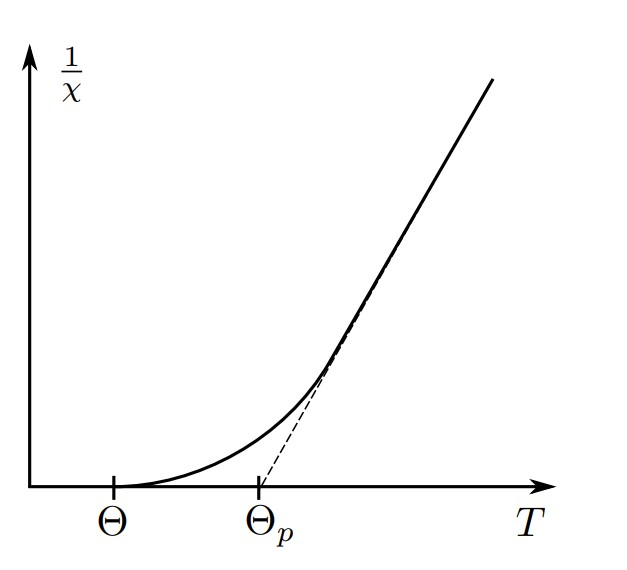
\includegraphics[width=0.5\linewidth]{"res/fig-chi_T.jpg"}
	\caption{Зависимость обратной величины магнитной восприимчивости от температуры}
	\label{fig:chi_T}
\end{figure}

Температуру фазового перехода парамагнетик–ферромагнетик называют температурой Кюри $\Theta_K$. Температурная зависимость магнитной восприимчивости у ферромагнетиков выше точки Кюри с удовлетворительной
точностью описывается законом Кюри-Вейесса:

$$\chi \propto \frac{1}{T - \Theta_p},$$
где $\Theta_p$ — параметр с размерностью температуры, называемый иногда парамагнитной точкой Кюри. Величина $\Theta_p$ близка к $\Theta_K$, но не совпадает
с ней. Непосредственно вблизи $\Theta_K$ закон Кюри–Вейсса нарушается. На
практике наблюдается зависимость, изображённая на рис. \ref{fig:chi_T}.
	
\subsection*{Ход работы}

В работе изучается температурная зависимость $\chi(T)$ гадолиния при
температурах выше точки Кюри. Выбор материала определяется тем,
что его точка Кюри лежит в диапазоне комнатных температур.

\begin{figure}[H]
	\centering
	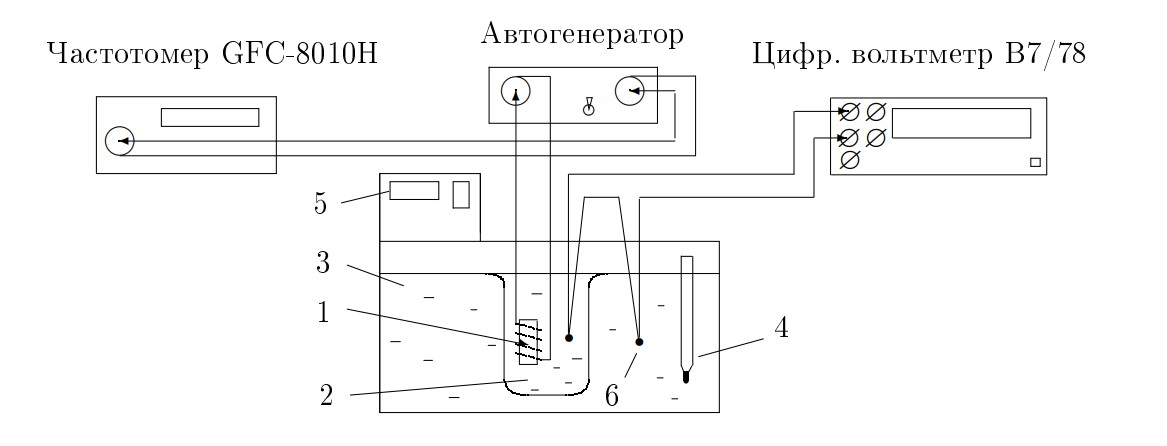
\includegraphics[width=1.1\linewidth]{"res/fig-scheme.jpg"}
	\caption{Зависимость обратной величины магнитной восприимчивости от температуры}
	\label{fig:scheme}
\end{figure}

Схема установки для проверки закона Кюри–Вейсса показана на
рис. \ref{fig:scheme}. Исследуемый ферромагнитный образец (гадолиний) расположен
внутри пустотелой катушки самоиндукции, которая служит индуктивностью колебательного контура, входящего в состав $LC$-автогенератора генератора колебаний с самовозбуждением).

Гадолиний является хорошим проводником электрического тока, а
рабочая частота генератора достаточно велика ($\sim 50$ кГц), поэтому для
уменьшения вихревых токов образец изготовлен из мелких кусочков размером около 0,5 мм. Катушка 1 с образцом помещена в стеклянный сосуд 2, залитый трансформаторным маслом. Масло предохраняет образец
от окисления и способствует ухудшению электрического контакта между отдельными частичками образца. Кроме того, оно улучшает тепловой
контакт между образцом и термостатируемой (рабочей) жидкостью 3 в
термостате. Ртутный термометр 4 используется для приближенной оценки температуры. Температура образца регулируется с помощью термостата 5.

Коэффициент самоиндукции катушки $L$ пропорционален магнитной
проницаемости $\mu$ заполняющей его среды: $L \propto \mu$. Тогда разность самоиндукций катушки с образцом $L$ и без него $L_0$ будет пропорциональна восприимчивости образца $\chi$:
$$L - L_0 \propto \mu - 1 = \chi .$$
При изменении индуктивности образца меняется период колебаний автогенератора:
$$\tau = 2\pi \sqrt{LC},$$
где $C$ — ёмкость контура автогенератора. Период колебаний в отсутствие
образца определяется самоиндукцией пустой катушки:
$$\tau_0 = 2\pi \sqrt{L_0C},$$
Отсюда находим
$$L - L_0 \propto \tau^2 - \tau_0^2$$
и, следовательно,
$$\chi \propto \tau^2 - \tau_0^2.$$
Из формул выше следует, что закон Кюри–Вейсса справедлив, если выполнено соотношение
$$\frac{1}{\tau^2 - \tau_0^2} = T - \Theta_p$$

\subsection*{Ход работы}

Исследуем зависимость периода колебаний $LC$-генератора от температуры образца, отмечая период колебаний $\tau$ по частотомеру, а температуру $T$ — по показаниям дисплея и цифровому вольтметру ($\Delta U$ с учётом знака).

Рассчитаем температуру $T$ образца с учетом показаний термопары. используя поправочный коэффициент для данной установки $k = 24 \frac{\text{град}}{\text{мВ}}$:
$$T = T_0 + k V$$
Все экспериментальные данные приведены в таблице \ref{tab:data}.

\begin{table}[H]
	\footnotesize
	\begin{tabular}{cccccc}
\toprule
$T_0,^{\circ} C$ & $V$, мВ & $\tau$, мкс & $T,^{\circ} C$ & $\chi$, мкс$^2$ & $1/\chi$, мкс$^{-2}$ \\
\midrule
14.1 & -0.0150 & 10.07 & 13.7 & 33.249 & 0.030 \\
16.0 & -0.0190 & 9.96 & 15.6 & 31.007 & 0.032 \\
18.0 & -0.0180 & 9.76 & 17.6 & 27.123 & 0.037 \\
20.0 & -0.0190 & 9.44 & 19.6 & 21.075 & 0.047 \\
22.0 & -0.0190 & 9.04 & 21.6 & 13.698 & 0.073 \\
24.0 & -0.0190 & 8.75 & 23.6 & 8.397 & 0.119 \\
26.0 & -0.0190 & 8.61 & 25.6 & 6.019 & 0.166 \\
28.0 & -0.0190 & 8.53 & 27.6 & 4.717 & 0.212 \\
30.0 & -0.0190 & 8.49 & 29.5 & 3.917 & 0.255 \\
32.0 & -0.0180 & 8.45 & 31.6 & 3.324 & 0.301 \\
34.0 & -0.0180 & 8.43 & 33.6 & 2.936 & 0.341 \\
36.0 & -0.0190 & 8.41 & 35.5 & 2.616 & 0.382 \\
38.0 & -0.0190 & 8.39 & 37.5 & 2.381 & 0.420 \\
40.0 & -0.0190 & 8.38 & 39.5 & 2.179 & 0.459 \\
\bottomrule
\end{tabular}

	\caption{Данные}
	\label{tab:data}
\end{table}

\begin{figure}[htb]
	\centering
\makebox[0pt][c]{%
\begin{minipage}[b]{.49\textwidth}
	\begin{figure}[H]
	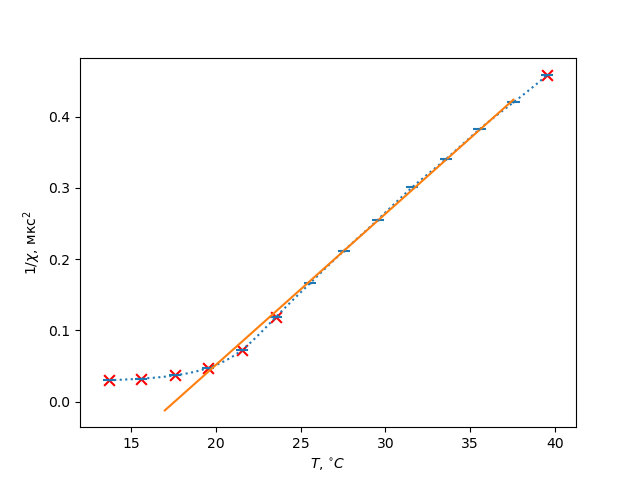
\includegraphics[width=1.3\linewidth]{"gen/fig-inv.pdf"}
	\caption{График зависимости $\frac{1}{\chi}\left(T\right)$}
	\label{fig:inv}
	\end{figure}
\end{minipage}
%
\hspace{0.5cm}
\begin{minipage}[b]{.49\textwidth}
	\begin{figure}[H]
	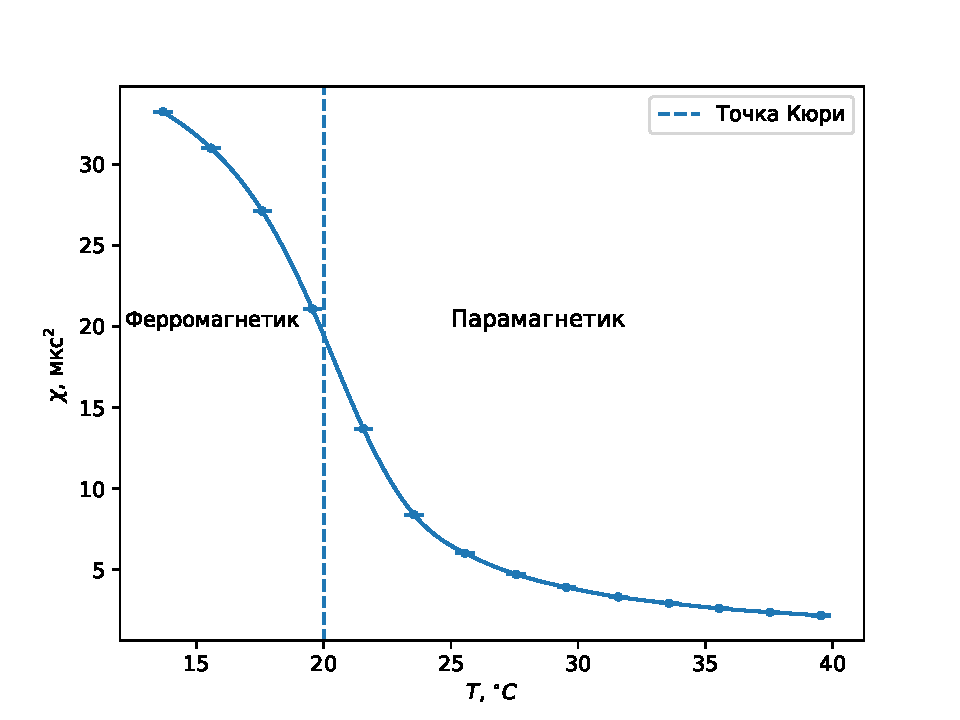
\includegraphics[width=1.3\linewidth]{"gen/fig-chi.pdf"}
	\caption{График зависимости $\chi\left(T\right)$}
	\label{fig:chi}
	\end{figure}
\end{minipage}
}%
\end{figure}

\begin{table}[H]
	\footnotesize
	\begin{tabular}{ccccccccc}
\toprule
$\overline{x}$ & $\sigma_x^2$ & $\overline{y}$ & $\sigma_y^2$ & $r_{xy}$ & $a$ & $\Delta a$ & $b$ & $\Delta b$ \\
\midrule
3.156e+01 & 1.597e+01 & 2.968e-01 & 7.204e-03 & 3.391e-01 & 0.021 & 0.000 & -0.373 & 0.009 \\
\bottomrule
\end{tabular}

	\caption{Обработка $\frac{1}{\chi}\left(T\right)$}
	\label{tab:mnk}
\end{table}

Из первого графика определим парамагнитную точку Кюри:
$$\Theta_p = ( 16.9 \pm 0.2 ) ^\circ C$$ 

Качественно из графика зависимости $\chi\left(T\right)$ найдем температуру Кюри:
$$\Theta_K \approx 20 ^\circ C$$

\subsection*{Вывод}

В работе было проведено изучение температурной зависимости магнитной восприимчивости ферромагнетика выше точки Кюри.

Из графика $\chi\left(T\right)$ с достаточно хорошей точностью получилось определить температуру Кюри гадолиния $\Theta_K \approx 20 ^\circ C$, что сходится с табличным значением $\Theta_K = 20.2 ^\circ C$.

Однако график $\frac{1}{\chi}\left(T\right)$ только качественно подтверждает теорию. Посчитанная погрешность также не может быть использована для объяснения расхождений. Вероятно сказалась некоторая систематическая погрешность.
\end{document}